\documentclass[twocolumn,11pt,a4]{article}
\usepackage[top=25truemm,bottom=30truemm,left=20truemm,right=20truemm]{geometry}
\usepackage{graphicx}
\begin{document}

\title{Propagation length of mid-infrared surface plasmon polaritons on polycrystalline gold}
\author{Nobuyoshi Hiramatsu, Satoshi Ashihara, Fumiya Kusa, Akinobu Takegami,\\ Kotaro Imasaka, Ikki Morichika, Kazuhiko Hirakawa, and Takuji Takahashi }
\maketitle

\section{Introduction}
Mid-infrared plasmonics on metal is beneficial for a number of applications including surface-enhanced spectroscopies, plasmonic circuit, supersensitive detection, thermal radiation control, and photoelectron emission\cite{Kusa2015}. 
Their functionalities rely on the degree of electric-field enhancement, induced by Surface Plasmons (SPs), namely, Localized Surface Plasmons (LSPs) and Surface Plasmon Polaritons (SPPs), which is strongly limited by loss rate or decay time of the SPs.

The SPs' loss is either radiative or irradiative. 
The former loss rate is the strength of coupling with propagating light that depends on the size and shape of the metal\cite{Kusa2014}. 
The latter microscopically originates from electron-electron scattering and electron-lattice scattering, reflecting the material morphology, being expressed by the dielectric constant of metal.
Propagation length of SPPs essentially characterize the latter loss, which measures the distance the SPPs diminish to $1/e$ of its initial value in power\cite{William}.

Gold is often used for a plasmonic material in visible and mid-infrared range, due to its high optical conductivity and stability under ambient condition\cite{Olmon}. 
However, the propagation length of mid-infrared SPPs on gold has not been measured as far as we know, whereas Shiba {\it et al.} reported on copper\cite{Shiba}.

In this study, we quantitatively investigated the propagation length of mid-infrared SPPs bound to a gold-air interface.
Material morphology of the gold was also correlatively discussed, indicating the strong influence to the propagation length. 
For direct evaluation of the propagation length, optical experiment was conducted using multiple sets of a waveguide with different lengths sandwiched by paired gratings on a sample, at $\mathrm{CO_2}$ laser wavelength. 
Annealing was applied to the sample twice at different temperatures for controlling the material morphology, and the optical experiments were conducted for the sample three times before and after annealing. 
For a each step, as soon as the optical measurement was done, Atomic Force Microscopy(AFM) probing were conducted for the characterization of the surface morphology of the sample. 
This study is not only valuable for the plasmonic applications to enhance the functionalities, but also for fundamental understanding of the loss mechanism.

The remainder of this paper is organized as follows: 
In Sec. \ref{sec:experiment}, experimental method and annealing procedure are described.
In Sec. \ref{sec:sample}, design and fablication techniques of the sample are illustrated.
In Sec. \ref{sec:surface_characterization}, surface characterization method and their results are introduced.
In Sec. \ref{sec:result}, the propagation length of SPPs measured by the optical experiment are shown.
In Sec. \ref{sec:discussion}, we discuss the relation between the propagation length and the material morphology of the sample.
In Sec. \ref{sec:conclusion}, we draw conclusions from the results of this research.

\section{Experiment}
\label{sec:experiment}
SPPs are coupled with propagating light within a grating structure which satisfies the phase-matching condition, as summarized in Ref.\cite{Koev},
\begin{equation}
k_{SPPgr}=k_0 sin\theta + \frac{2n\pi}{d},
\label{eq:phase-match}
\end{equation}
where $k_{SPPgr}$ and $k_0=2\pi/\lambda_0$ is the wave vector of SPPs on a grating and propagating light, $\lambda_0$ is the wavelength of the propagating light, $\theta$ is incident angle, $d$ is grating pitch, and $n$ is a positive or negative integer. 

In this study, SPPs were excited by incident light with a grating (in-coupler), to propagate along a waveguide until they reach another grating (out-coupler) to radiate. The out-coupled power emitted from the out-coupler is considered to be proportional to the power of the SPPs that flow into the out-coupler, in the assumption that the efficiency of SPP-light coupling is steady among all couplers, while maintaining the incident light in power. It follows that, the out-coupled light decreases at the same rate to the SPPs, as the distance between the in-coupler and out-coupler increases. We calculated the distance that the out-coupled power falls to 1/e, depending the length of the waveguides: that is, equivalent to the propagation length of the SPPs.  

Fig. \ref{fig:Experiment}(A) shows schematic of experimental setup. A $\mathrm{CO_2}$ laser was used for a mid-infrared light source generating linearly polarized light at wavelength of 10.6$\mu m$. The power was controlled by Pulse Width Modulation in radio frequency.
P-polarized light was incident into the in-coupler at a certain angle that fulfills Eq. \ref{eq:phase-match} with n=1, being loosely collimated by a spherical mirror with R=400mm. The out-coupled light was collected by a power meter using a spherical mirror with R=150mm. 
An aperture was arranged in front of the power meter, being optical conjugate with the out-coupler in the sample which is attached with a xyz-stage on a rotational table. We also used a He-Ne laser for a guide laser, to be coupled with the mid-infrared light passing through a CaF substrate which behaves as a partial mirror in both visible and mid-infrared ranges.

Annealing was applied to the sample twice on a hotplate in Argon atmosphere, for increasing grain size on the surface of the waveguides\cite{Nogues}. In the first annealing process, the sample was heated at 600$^\circ\mathrm{C}$ for 20min, and gradually cooled on the hotplate at room temperature. In the second annealing, the sample was heated at 700$^\circ\mathrm{C}$ for 16min, cooling down in the same way.


 \begin{figure}[!htbp]
   \begin{center}
    \includegraphics[width=\hsize]{./RCWA_Rplot.eps}
    \caption{(A) Schematic of experimental setup. (B) Gratings and waveguide design. (C) Reflection efficiency on a grating with pitch $15\mu m$ and duty cycle 50\%, calculated by RCWA.}
     \label{fig:Experiment}
   \end{center}
\end{figure}

\section{Sample}
\label{sec:sample}
We designed multiple waveguides with lengths ranging from 3 to 11mm with a 2mm step, sandwiched by gratings with length $1.0mm$ as shown in Fig. \ref{fig:Experiment}(B). A width of the waveguide and the in-coupler is $0.5mm$, while the out-coupler has a width of $1.5mm$. Both of the in-coupler and out-coupler have a rectangular profile with pitch of $15\mu m$ in duty cycle 50\%. Each of the waveguides is parallelly aligned with a spacing $1.5mm$. The waveguides and swelling part of gratings are optimized to be 800nm higher than the gold base, as illustrated bellow.

Grating depth is reported as significantly influential for the SPP-light coupling efficiency\cite{Koev}\cite{Justin}. 
To estimate the optimized grating depth for strong SPP-light coupling that results in high signal-to-noise ratio of the optical experiment, we conducted a numerical calculation of  the reflection efficiency on a grating, based on Rigorous Coupled-Wave Analysis (RCWA)\cite{Leveque}. 
A grating with a rectangular profile with pitch of $15\mu m$  in duty cycle 50\%, the dielectric function of polycrystalline gold for a grating material, and incident light as a plane wave propagating in vacuum at wavelength of 10.6$\mu m$, are assumed.
Fig. \ref{fig:Experiment}(C) shows clear dips on the reflection efficiency at where the grating depth is roughly from 0.2 to 1.3$\mu m$, due to energy conversion from propagating light to SPPs, indicating SPP excitation on the grating.
We expected the effective coupling efficiency takes the maximum value around the depth 0.8$\mu m$ in this experiment, taking the certain angular divergence of incident light into consideration.
The height of a grating structure was designed to be 0.8$\mu m$, in a reasonable agreement with a previous report estimating optimum grating depth for a rectangular grating to be 10\%-15\% of the wavelength in mid-infrared range\cite{Justin}.

The sets of gold gratings and a waveguide were fabricated on a gold base layer on a glass substrate, by using electron beam lithography, thermal evaporation, and lift-off process. The gold base with thickness 200nm was thermally evaporated on a glass substrate with a Chromium adhesion layer with thickness 5nm, after cleaning the substrate with acetone and ethanol. Then, EB resist (OEBR-CAP112PM, TOK) was spin-coated on the base with thickness 1700nm to be exposed in electron beam for development. Finally, gold with thickness 800nm was evaporated on the top of the developed resist, and the resist was lifted off using acetone. The whole fabrication process was conducted at room temperature. During the evaporation, we maintained the evaporation rate of gold to be 0.4nm/s, and the pressure inside the vacuum chamber less than $3\times10^{-5}$Torr. 

\section{Suface Characterization}
\label{sec:surface_characterization}
Isotropic deposition of gold and flat surface were confirmed. The surface state changes drastically after annealing as shown in Fig. \ref{fig:morphology}. Surface roughness is estimated as 3.58nm for the as-grown sample, 16.2nm for the sample annealed at 600$^\circ\mathrm{C}$, and 18.3nm for the sample annealed twice at 600$^\circ\mathrm{C}$ and 700$^\circ\mathrm{C}$, by calculating two-dimensional root mean squares of deviations in height data.  As annealing applied, the surface roughness increased.
The gratings were not significantly transformed after the annealing. However, there appear to be pinholes on the surface of waveguide with $1\mu m$ order as the annealing applied.

For detailed characterization of the surface morphology, we identified crystal grains on the surface based on watershed algorithm\cite{Petr}, to estimate diameter of the crystal grains in the assumption that a grain is close to spherical shape. Average grain diameter corresponds 70nm, 190nm, and 180nm, respectively for the as-grown sample, the sample annealed at 600$^\circ\mathrm{C}$, and the sample annealed twice at 600$^\circ\mathrm{C}$ and 700$^\circ\mathrm{C}$.
The grain size has significantly increased as the first annealing at 600$^\circ\mathrm{C}$ was applied, whereas there does not seem to be grain enlargement by the second annealing at 700$^\circ\mathrm{C}$, relying on the AFM measurement.

 \begin{figure}[!htbp]
   \begin{center}
    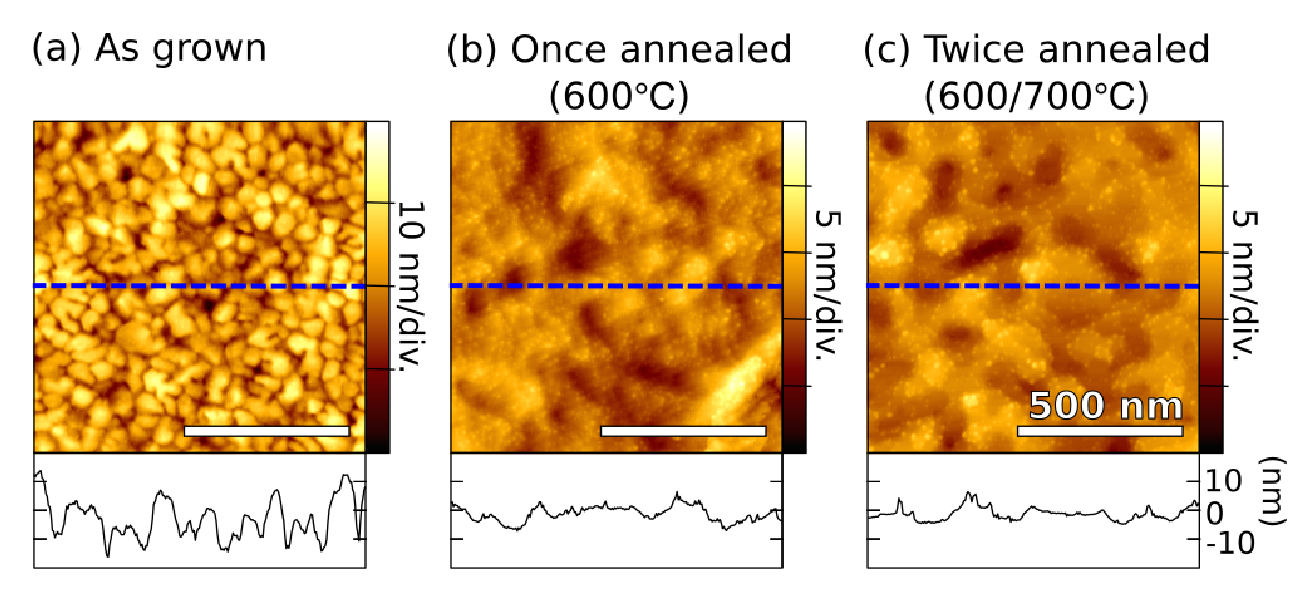
\includegraphics[width=\hsize]{./morphology.eps}
    \caption{Height plots on the surface of waveguides based on AFM. Crystal grain diameter is estimated to be 70nm for the as-grown sample (a), 190nm for the sample annealed at 600$^\circ\mathrm{C}$ (b), and 180nm for the sample annealed twice at 600$^\circ\mathrm{C}$ and 700$^\circ\mathrm{C}$ (c).}
    \label{fig:morphology}
   \end{center}
\end{figure}

\section{Result}
\label{sec:result}
Fig. \ref{fig:propagation_length} shows the power out-coupled from the propagating SPPs along the waveguides with a different length L, measured for each of the sample before and after annealing.
Each of the out-coupled power is normalized for ignoring systematic errors, originated from a laser-power drift and a minor shift of SPP-light coupling efficiency on the gratings by the annealing.
By the method of least squares, they are fitted with exponential functions. Low degree of the inclination indicates longer propagation length. The propagation length is evaluated with a standard error as 9.01$\pm$0.26mm for the as-grown sample, 11.96$\pm$0.42mm for the sample annealed at 600$^\circ\mathrm{C}$, and 14.74$\pm$0.65mm for the sample annealed twice at 600$^\circ\mathrm{C}$ and 700$^\circ\mathrm{C}$.
Evidently, the propagation length increased as annealing applied.

 \begin{figure}[!htbp]
   \begin{center}
    \includegraphics[width=\hsize]{./propagation_length.eps}
    \caption{Measured power out-coupled from the propagating SPPs along the waveguides with a different length L, in arbitrary unit, as shown in the inset. The propagation length of the mid-infrared SPPs is evaluated with a standard error as 9.01$\pm$0.26mm for the as-grown sample, 11.96$\pm$0.42mm for the sample annealed at 600$^\circ\mathrm{C}$, and 14.74$pm$0.65mm for the sample annealed twice at 600$^\circ\mathrm{C}$ and 700$^\circ\mathrm{C}$.}
       \label{fig:propagation_length}
   \end{center}
\end{figure}

\section{Discussion}
\label{sec:discussion}
The propagation length of mid-infrared SPPs on gold were precisely measured at $\mathrm{CO_2}$ wavelength. Propagation length of 12.3mm was calculated by the dielectric constant of polycrystalline gold at the wavelength measured by Palik {\it et al.}\cite{Palik}, using a following equation\cite{William}.
\begin{equation}
 \delta_{SPP} = \lambda_0 \frac{(\epsilon'_m)^2}{2\pi\epsilon''_m} (\frac{\epsilon'_m+\epsilon_d}{\epsilon'_m \epsilon_d})^\frac{3}{2},
\label{eq:propagation_length}
 \end{equation}
where $\delta_{SPP}$ is the propagation length of SPPs, $\epsilon_m=\epsilon'_m+i\epsilon''_m$ and $\epsilon_d=1$ are dielectric function of metal and air which behaves as a dielectric. 
This estimation does not contradict the propagation length for each of the samples, measured before and after the annealing. 

Comparing the as-grown sample with the sample annealed at $600^\circ\mathrm{C}$, we found the increased propagation length and an enlargement of the crystal grains. 
The longer propagation length can be described by reduction of mean free path for electrons scattered by grain boundaries, that results in different dielectric constants.\cite{Jens}
An additional loss mechanism was studied in Ref. \cite{Kuttge}, that SPPs scatters due to inhomogeneities of free electron gas by introduction of grain boundaries. 
Here, we confirmed the loss reduction of SPPs in mid-infrared range, due to enhancement of morphology as annealing applied.

After the additional annealing at $700^\circ\mathrm{C}$, the average grain diameter does not appear to be enlarged, although the propagation length increased considerably. 
We think this mismatch occurred, mainly due to an inherent characteristic of the AFM that the internal state may not be perfectly measured.
AFM is only available for measuring surface state, overlooking internal imperfections such as voids generated in the deposition process, while the electric field of SPPs penetrates into the gold surface reflecting the internal state. 
In practice, there is also a difficulty to estimate grain size by analyzing the surface, due to a free parameter which is arbitrary defined in the watershed algorithm.
In any case, the elongated propagation length was demonstrated as annealing applied, which is relevant with the material morphology.

Annealing is convenient for controlling material morphology\cite{Nogues} without damaging the sample in relatively low temperature range. Its minor side effects are noted as follows.
Pinholes were generated on the surface of waveguides as the annealing applied. However, influence of increased surface roughness, contributed from the generation of pinholes, is negligible compared with the enlargement of crystal grains. Surface roughness is regarded to reduce the propagation length of SPPs\cite{Mills}, however, the propagation length increased on the contrary after the annealing.
Optimum incident angle to excite SPPs within a grating was shifted by up to 0.5$^\circ$ after the annealing.
This angle shift is supposed to be slightly different for each of the gratings, that results in the increased standard error for the measured propagation length.

The SPP-light coupling efficiency within a grating was estimated as 18\% at the maximum, in the experiment, by measuring a anomalous dip on reflection efficiency.
This efficiency is sufficiently high for precisely evaluating the propagation length of the SPPs, and no significant change was confirmed in the efficiency after the annealing.

As mentioned above, we demonstrated the elongated propagation length of mid-infrared SPPs as annealing applied, reflecting material morphology, mainly due to an enlargement of crystal grains that results in different dielectric constants. 
This result has a positive impact on plasmonics and its applications demonstrating loss reduction by annealing.

\section{Conclusion}
\label{sec:conclusion}
For the first time, we precisely measured the propagation length of SPPs on polycrystalline gold in mid-infrared range. 
The measured propagation length was in good agreement with an estimation by the dielectric constant of polycrystalline gold.
We demonstrated the propagation length of mid-infrared SPPs can be significantly increased as annealing applied, resulting in a long propagation length more than 14mm. 
It is confirmed that the material morphology of gold is related with the propagation length of SPPs. 
Direct quantitative evaluation of the irradiative loss is beneficial for the sake of both fundamental plasmonics and its applications to enhance the functionalities.

\section*{Acknowledgement}
The sample was fabricated at VLSI Design and Education Center (VDEC), the University of Tokyo.
The author thank Dr. Tayama for fruitful discussions and helpful advices.

\bibliographystyle{unsrt}
\bibliography{./Reference}

\newpage

\end{document}